\documentclass[11pt,a4paper,titlepage]{article}

\usepackage[spanish,es-nodecimaldot]{babel}
\usepackage[utf8]{inputenc}
\usepackage[T1]{fontenc}
\usepackage[margin=0.9in]{geometry}
\usepackage{amsmath,amsfonts,graphicx,float,booktabs,url,siunitx}
\usepackage[font=footnotesize,labelfont={sf,bf},textfont=sf]{caption}
\usepackage[usenames,dvipsnames]{xcolor}
\usepackage[plainpages=false,pdfpagelabels,hypertexnames=false,hidelinks]{hyperref}
\graphicspath{{./Img/}}
\captionsetup{width=0.7\linewidth}

\makeatletter
\DeclareMathSizes{\@xpt}{\@xpt}{6}{5}
\makeatother

\title{\Huge\textbf{El problema de la cuantización de la interacción gravitatoria}}
\author{\textsf{Iyán Méndez Veiga}\\ \textsf{Víctor Rodríguez Bouza}}
\date{\texttt{TRG 2015-2016}}

\newcommand{\HRule}{\rule{\linewidth}{0.5mm}} % Para el título

\addto{\captionsspanish}{\renewcommand{\refname}{\vskip -1cm}} % Para que BibTeX no ponga su título propio.
\setlength{\parskip}{1em} % Cambia aquí la separación a la que te guste pero lo de usar \\ + \par es mala práctica, a mí me salen todos warnings con underfull y tal

% -------------------------------------------------------------

\begin{document}
% Portada provisional. Luego ya la haremos más guapa si hay tiempo (que lo dudo)
%\maketitle
\begin{titlepage}
\begin{titlepage}
\begin{center}

% Upper part of the page. The '~' is needed because \\
% only works if a paragraph has started.

% Title
\HRule \\[0.4cm]
{ \huge \bfseries El problema de la cuantización\\de la interacción gravitatoria. \\[0.3cm] }

\HRule \\[1.5cm]

\textsc{\Large Teoría de la Relatividad General}\\[1cm]

\vfill

% Bottom of the page
\large{\textsf{Iyán Méndez Veiga y Víctor Rodríguez Bouza}}


\textmd{Facultad de Ciencias \\
Universidad de Oviedo}

\texttt{Curso 2015-2016}



\end{center}
\end{titlepage}

\end{titlepage}


\newpage
\tableofcontents
\newpage


\begin{abstract}
La fuerza gravitatoria es una de las cuatro interacciones que gobiernan el universo. Durante todo el siglo XX, los modelos de la misma han recibido un empujón gracias a la teoría de la relatividad general de Albert Einstein, pero diversos problemas han aflorado a finales de la centuria. En tal situación, la cuantización de la gravedad se hace necesaria. En este trabajo explicamos los motivos por los que los investigadores de finales de siglo se ven obligados a tal esfuerzo. A continuación, explicamos la esencia de las principales alternativas que están en estudio para resolver el problema: \textit{Loop Quantum Gravity}, teoría de cuerdas, o aproximaciones covariantes entre otras. Finalmente exponemos las últimas novedades en el campo, unas conclusiones de más de medio siglo cuantizando la gravedad y las perspectivas futuras.
\end{abstract}


\section{Introducción. ¿Por qué es necesaria la cuantización de la gravedad?} % Víctor

\subsection{Aproximación histórica}

Para los antiguos astrónomos, el cielo estrellado escondía misterios que les apasionaban. ¿Por qué el Sol, que tanto calor nos da, y permite a nuestros cultivos florecer, aparece al amanecer y se esfuma al atardecer? ¿Qué son las estrellas? ¿Luces «pegadas» sobre una esfera perfecta, como diría Aristóteles? ¿O algo más? ¿Hay gente acaso viviendo en las estrellas? ¿Podemos ir a la Luna? Obviamente, la bóveda celeste era una fuente casi inagotable de inspiración: origen de multitud de leyendas y narraciones mitológicas.

Uno de los procesos que ya intrigaba en la antigüedad eran los movimientos de cuerpos como Marte u otros, que eran \textit{erráticos} (¡el que menos!). Como es bien sabido, la evolución de la investigación en estos campos derivó en distintas concepciones de distribución de los astros en el cosmos. Aristóteles, Ptolomeo y otros ofrecieron sus propuestas respecto al por qué de estos movimientos. Sería más adelante, durante la Revolución Científica del Renacimiento cuando el modelo heliocéntrico de Aristarco rescatado por Copérnico se asentara firmemente, sobre todo en el siglo XVII. \textbf{Kepler} fue el primero que dio un análisis físico (en el sentido que hoy lo consideraríamos) sobre el movimiento de los cuerpos del sistema solar. Sin embargo, la humanidad tuvo que esperar algunos años más para que llegara la primera concepción científica (en el sentido actual) sobre la fuerza que origina tales desplazamientos: \textbf{la gravedad}.

\textit{Sir} Isaac Newton ofreció en el siglo XVII un modelo matemático de lo que bautizó como fuerza gravitatoria, basado en su cálculo de fluxiones (cálculo diferencial) y la idea mejorada del movimiento galileano. Ésta interpretación es considerada como la proposición de Newton para los modelos sobre gravedad en la «concepción clásica de la física». Es esencialmente lo que hoy en día se entiende por \textbf{gravedad newtoniana}.

Éste modelo de fuerza gravitatoria permitió entender esta interacción tanto en cuerpos diminutos, como en planetas y estrellas muy masivas. Habilitó la posibilidad de avance del estudio de la mecánica celeste, interpretando las leyes de Kepler como particularizaciones de su modelo y cosechando numerosos éxitos experimentales. Un ejemplo es el descubrimiento de Neptuno, que se hizo tras haberse hallado perturbaciones en el período de la órbita de Urano. Entonces, Urbain Le Verrier predijo la existencia de un nuevo planeta, empleando la teoría de Newton. Tal cuerpo afectaría a la órbita de Urano y permitiría explicar tales órbitas. Su colega Gottfried Galle descubriría más tarde a Neptuno tal y como Le Verrier había dicho.

Pero no sería la única órbita que se escapara a las predicciones iniciales de la gravedad newtoniana. El propio Le Verrier descubrió que, pese incluso contando con la acción del resto de planetas (además del Sol) sobre el planeta Mercurio, había extraños resultados experimentales en su órbita que no cuajaban con las predicciones newtonianas, concretamente, su precesión en el perihelio. En un alarde de innovación, Le Verrier, basándose en que la teoría de Newton era correcta, propuso en 1859 la hipótesis de un nuevo planeta entre Mercurio y el Sol: Vulcano. Sin embargo, éste nunca se descubrió.

Albert Einstein trabajaba en una oficina de patentes en Berna (Suiza) cuando postuló su teoría de la relatividad especial. Debido a su trabajo monótono y repetitivo, podía abstraerse en el mismo y hacer experimentos mentales físicos para probar sus ideas. Cuando se dedicó a hacer compatible la teoría de la relatividad especial con la gravedad newtoniana se dio cuenta de numerosas problemáticas que lo forzaron a desarrollar un nuevo marco en los comienzos del siglo XX para la interacción gravitatoria. Un marco no cuántico, pero que sí incluyera la relatividad especial y la gravedad clásica. Dicho modelo acabaría llevando el nombre de \textbf{teoría de la relatividad general}.\footnote{Cabe decir que antes de que Einstein presentara su artículo, Hilbert llegó a dar con una ley de gravitación completamente igual a la del primero de forma independiente. La publicación el 25 de noviembre de 1915 en la Academia Prusiana de Ciencias por parte de Einstein de sus resultados generó una situación incómoda entre ambos. Sin embargo, Hilbert acabó aceptando lo sucedido, y cedió todo el protagonismo a Einstein en su obra maestra. En el futuro, Einstein y Hilbert se considerarían el uno al otro como colegas científicos, sin recuerdo de esos «nubarrones» (\cite[p.~49-50]{teoriaperfecta}).}

Como teoría científica que se precie, debía poder ponerse a prueba, y así fue. Una de las comprobaciones de su utilidad está en que con este modelo es posible interpretar el extraño fenómeno de la órbita de Mercurio, por ejemplo. Otras pruebas de la teoría, como la observación de estrellas tras el Sol durante un eclipse, confirmaron su validez.

Las ecuaciones de Einstein (como se conoce a las principales relaciones de éste modelo) son una herramienta muy potente para entender el funcionamiento general del cosmos. Y muy liosa, también. Einstein fue, obviamente, el primero que se lanzó al empeño de resolverlas, buscando un \textbf{modelo adecuado} de la realidad que nos rodea surgido de ellas.

El resultado al que llegó fue una solución en la que aplicó el conocimiento (muy limitado para nosotros) que en 1916 se tenía del universo cercano: supuso que el universo estaba repleto de masa distribuida de forma uniforme. Dadas esas hipótesis, llegó al extraño resultado de que tal universo debería empezar eventualmente un proceso de evolución, de cambio, de modo que en un determinado momento, el universo no siguiera siendo estático a escala macrocósmica. Esta posibilidad fue despreciada por Einstein, quien derrotado por su intuición física y sus ideas preconcebidas \textbf{introdujo una constante en las ecuaciones} cuyo único fin era contrarrestar los efectos de la masa sola en el universo. De este modo, se podía tener un universo estable, en un equilibrio entre las fuerzas de la masa del mismo y lo que las contrarrestaba la constante. Dicho valor recibió el nombre de \textbf{constante cosmológica} y es uno de los pilares hoy en día de la cosmología moderna. Pero, ¿qué es la cosmología en esencia? La cosmología, en su acepción científica, es una disciplina dependiente de la física que estudia el origen, evolución y destino del universo en su totalidad empleando modelos físicos para tal fin. Será durante el siglo XX cuando recibirá su impulso principal, gracias a la teoría de la relatividad general.

En los años siguientes numerosos modelos surgieron a raíz de las conocidas como ecuaciones de Einstein: el modelo De Sitter, el de Lemaître, el de Friedmann, etcétera. Las pruebas experimentales acabaron demostrando, a través del corrimiento al rojo (o \textit{redshift}) que \textbf{el universo no es estático y} que \textbf{se encuentra en expansión} gracias a Hubble, Ryle y otros que rebatieron las tesis estacionarias de Hoyle y compañía.

A lo largo de lo que quedaba del siglo XX, los estudios sobre relatividad general aumentaron, tratando temas muy diversos: el Big Bang y la evolución hasta nuestros días, búsqueda de otras pruebas experimentales (como ondas gravitacionales), temas relacionados con materia oscura o energía oscura o incluso surgieron algunos problemas que apuntarían a una posible cuantización de la teoría para solventarlos (empresa que hoy en día sigue). Podríamos estar discutiendo durante muchos párrafos todo ésto, pero ese no es el fin de este texto.

En 1947, y justo al acabar la carrera, Bryce DeWitt tuvo la oportunidad de conocer a Wolfang Pauli, aprovechando la ocasión para decirle que estaba trabajando en la cuantización del campo gravitatorio. A DeWitt le resultaba incomprensible que las dos teorías científicas más revolucionarias del siglo XX (la física cuántica y la relatividad general) no tuvieran ninguna relación entre sí. Pauli, sin embargo, no estaba de acuerdo con que DeWitt empleara su tiempo en ello: «ese problemas al que apuntas es muy importante, pero para resolverlo se necesitará a alguien realmente listo»\footnote{\cite[p.~230]{teoriaperfecta}.}. Sin menoscabo de la inteligencia o de la capacidad de DeWitt, el tiempo ha demostrado lo acertado que estaba Pauli en tal ocasión.

Los primeros pasos hacia tal hipotético encuentro entre Einstein y la mecánica cuántica los daría Paul Dirac. Sería él, quien junto a otros como Klein-Gordon propiciaran el advenimiento de la teoría cuántica de campos (\textit{Quantum Field Theory} o QFT) gracias a la ecuación de Dirac. Ésto posibilitó (además de otras importantes contribuciones) reencontrar las nuevas teorías sobre partículas con la relatividad especial de Einstein, acercándolas a la relatividad general un poco más.

Quiere ser la historia irónica, y el hecho es que a Dirac las nuevas teorías de física de partículas que acabarían dando el hoy famoso modelo estándar (\textit{Standard Model}, SM) no le gustaban ni un pelo. Pese a agregar a las fuerzas débil y fuerte, y ofrecer predicciones que se mostrarían certeras, lo que incordiaba a Dirac era la «suciedad formal» que tenía la teoría en forma de renormalizaciones. Dirac era un hombre que apreciaba lo matemático, las relaciones, la realidad que subyacía a los experimentos mundanos de laboratorio.

En los últimos años de su vida, Dirac acabó aislado de la comunidad científica por su negativa a aceptar los logros de la física cuántica. No cesó de instigar a sus compañeros a buscar una teoría más general que no necesitara de las \textit{abyectas} renormalizaciones. Tampoco le sorprendió nada que DeWitt, eventualmente hallara problemas de renormalización en su cuantización de la gravedad. Dirac creía que para unificar ambos mundos sería necesaria una comprensión más profunda de la teoría cuántica.

DeWitt, mientras, se dedicó a intentar cuantizar el gravitón, que sería la partícula que «transportaría» (mediaría) la interacción gravitatoria: empresa más ardua de las que nunca imaginara, y que ya habían intentado otros como Matvei Bronstein, el propio Paul Dirac, Richard Feynmann, Wolfgang Pauli o Werner Heisenberg. Los esfuerzos que él y otros a la par como Dennis Sciama (Óxford), Stanley Deser (Boston) o Abdus Salam (Paquistán) estaban llevando a cabo se pusieron en común en 1974, cuando se realizó un simposio sobre gravedad cuántica en la Universidad de Óxford.

Aunque la comunidad científica vivía una relativa euforia (el ya existente CERN no paraba de confirmar los resultados que el modelo estándar de física de partículas predecía), según fueron pasando los ponentes ese clima de éxtasis se fue esfumando. De acuerdo con Wolfgang Pauli, se podía escuchar cómo los organizadores del evento murmuraban inquietos: «lo que Dios ha separado, que no lo una el hombre»\footnote{\cite[p.~242]{teoriaperfecta}.}.

La gravedad cuántica parecía estar en un callejón sin salida y la reconciliación de la fuerza gravitatoria con las otras tres parecía imposible, y el simposio de Óxford fue la viva imagen de ello... en su \textit{inmensa} mayoría. El evento habría significado la viva imagen de la derrota de no ser por la conferencia que diera el científico de la Universidad de Cambridge Stephen Hawking. Sería éste quien mostrara un vínculo entre la gravedad de Einstein y la física cuántica a través de un modelo de los agujeros negros.

Lo que se descubrió, en resumen, en las postrimerías del siglo XX fueron una serie de problemas que aparecían con la relatividad general cuando se las aplicaba a algunos casos \textit{extremos}. Un ejemplo de éstos casos podría ser mismamente el agujero negro. De este modo sería que la comunidad científica vería como necesaria la cuantización de la gravedad como solución a bastantes de ellos. También existen alternativas \textit{clásicas} de relatividad general, que intentan bordear problemas como la materia oscura o la energía oscura. Ejemplos de ellas son las MOND o TeVeS, pero no son objeto de estudio de este texto.

En este momento, resulta más adecuado para los fines del trabajo abandonar la perspectiva histórica y abordar los problemas de la relatividad general y la necesidad de la cuantización desde un punto de vista más \textit{aislado}. Veámoslo.


\subsection{La necesidad de la gravedad cuántica.}
\par Como vimos en el epígrafe anterior, un conjunto de problemáticas y motivos empezaron a surgir a finales del siglo pasado que apuntaban a la necesidad de una teoría cuántica de la gravedad. En este apartado veremos cuáles han sido los principales argumentos que han sido esgrimidos hasta la actualidad para ello.

\begin{description}
  \item[Completitud formal.]{Como dijimos en el subapartado histórico, uno de los principales motivos para la búsqueda de una teoría \textit{superior} (entendiendo por ello que contenga a ambas) a la teoría de la relatividad general y la mecánica cuántica es la «completitud formal». Por ésto entendemos que la existencia de dos teorías con una confirmación experimental tan reafirmada como la gravedad de Einstein y la física cuántica y de aplicación al universo entero incita a pensar en su posible vínculo. Sería algo parecido a la motivación de DeWitt.

  Pero no es necesario quedarnos con esa idea tan abstracta del motivo: es muy sencillo encontrar experimentos mentales, como los usados normalmente en mecánica cuántica, para ver un posible vínculo. Veamos un ejemplo postulado por Feynman en la conferencia de Chapel Hill de 1957.

  Imaginemos una suerte de experimento de Stern-Gerlach en el que conseguimos eventualmente dos partículas en un estado de superposición de espín $+1/2$ y $-1/2$. Hagamos ahora pasar esas dos partículas por dos contadores (algo que las partículas puedan accionar), de modo que uno de ellos esté conectado a una bola de dimensiones macroscópicas que se mueva al activarlos. En tal caso, la superposición de las partículas será transferida a la bola, que podrá estar en dos posiciones distintas a la vez... pero esto quiere decir que el \textit{campo gravitatorio está en una superposición} también. Si hacemos que el campo de esa bola afecte a otras mayores o más distantes, para comprender la interacción gravitatoria de éstas deberemos seguir la cadena de fuerzas e interpretar en última instancia de un modo mecano-cuántico el campo gravitatorio.\footnote{Cabe resaltar que una comprobación experimental de estos «juegos mentales» no existe, pero sirven para expandir el campo de conocimiento y buscar una teoría más «completa». Así es en parte cómo avanza la ciencia.}}

  \item[Unificación.]{Las teorías de unificación de las interpretaciones de las fuerzas han resultado muy útiles en física de partículas, llevando a resultados experimentales muy contrastables. Haciendo la extensión, parecería lógico pensar que podría llegar a conocerse una teoría más general que incluyera las cuatro interacciones fundamentales, y tal modelo necesitaría de la cuantización del campo gravitatorio.}

  \item[Existencia de singularidades.]{En el electromagnetismo clásico se suelen dar singularidades (es decir, puntos donde los campos o determinadas funciones \textit{no existen}) que han sido resueltas en la electrodinámica cuántica. Cabría esperar que las singularidades de la teoría de la relatividad general (Big Bang, agujeros negros...) se pudieran resolver en una teoría cuántica de la gravedad.}

  \item[El problema del tiempo.]{Aunque tanto la gravedad de Einstein como las teorías cuánticas ofrecen resultados experimentales veraces, poseen una concepción de tiempo completamente distinta. En la mecánica cuántica, el tiempo se considera absoluto algo que con la incorporación de la rel. especial cambió: en teoría cuántica de campos es el espaciotiempo el que es absoluto. Sin embargo, ninguna de las dos tiene en cuenta las dilataciones temporales debidas al cambio del espaciotiempo por la masa-energía. Obviamente, ambas interpretaciones no pueden ser ciertas a la vez, y se hace necesaria una interpretación más general que esclarezca la problemática. Al hecho de que esta hipotética teoría no dependa de un tiempo \textit{fijo} se le suele llamar «independencia del fondo» o «\textbf{\textit{background independence}}».}

  \item[Incompletitud del modelo estándar.]{El \textit{Standard Model} ha sido uno de los mayores logros de la física desde mediados del siglo XX. Sin embargo, no es una teoría científica como la mecánica cuántica: es una explicación parcial de las interacciones entre partículas que no pretende ser una teoría completa. Es decir, una \textit{aproximación} a unas leyes generales que subyacen a los fenómenos y que permitirían una explicación más simple y mejor globalmente que la que ofrece el SM. Ésto no quita para que haya hecho predicciones maravillosas que han podido ser fantásticamente contrastadas, ni tampoco es posible quitarle relevancia a que ha sido capaz de dar una interpretación para tres de las cuatro fuerzas fundamentales.

  Una de las carencias del modelo estándar es que no es válido a energías arbitrariamente elevadas. Si éstas son altas, el modelo estándar deja de ser una teoría cuántica de campos consistente, debido a varios motivos (polos de Landau, inestabilidad del potencial efectivo, etcétera). No es lo único: tampoco se entiende la masa del bosón de Higgs, la cual debería ser considerablemente mayor.

  En este contexto es natural plantearse si estas carencias a tal régimen de energías no serán debidas a la ausencia de la interacción gravitatoria en el modelo, aparte de otras explicaciones (como las teorías de supersimetría, por ejemplo). Concretamente, se espera que la hipotética influencia de la gravedad en el modelo estándar ocurra a energías elevadas, cercanas a las de la escala de Planck ($l_P\sim\SI{1.6e-33}{cm}$, $t_P\sim\SI{5.4e-44}{s}$ y $m_P\sim\SI{1.2e19}{GeV.c^{-2}}=\SI{2.2e-5}{g}$). Debido a que el SM es una teoría \textit{cuántica} de campos, necesitaríamos cuantizar la gravedad de Einstein para introducirla en el mismo.

  Cabe destacar que la lejanía de los regímenes de energías que hemos citado son un bache para el avance de la gravedad cuántica, ya que se encuentran lejos de nuestras posibilidades factibles hoy en día. Tampoco tenemos un acceso «fácil» a fenómenos astrofísicos en los efectos de la cuantización se pudieran apreciar. Esto complica mucho la búsqueda de tal teoría, puesto que no se tienen resultados experimentales «gravitocuánticos» disponibles que sean precisamente los que tengamos que interpretar.}

  \item[Existencia de resultados semiclásicos.]{Otro motivo viene de las aproximaciones a la teoría cuántica de la gravedad que se han venido haciendo, como la interpretación de Hawking de la temperatura de los agujeros negros (efecto Hawking). Pese a no tener comprobación empírica, resulta ilusionador que existan resultados basados en teoría cuántica de campos en espaciotiempos curvos que necesiten de ésta, de la mecánica cuántica, tengan una hipotética explicación. Además, ofrecen a nuestros colegas experimentales un reto: la medición de tales posibles predicciones. Que haya este tipo de modelos físicos es otro motivo más que incentive la búsqueda de una interpretación general que una los mundos cuántico y de la relatividad general.

  Uno de los ejemplos más característicos, como ya hemos dicho, es la interpretación de Hawking de los agujeros negros. Bajo la teoría cuántica de camos en un espaciotiempo curvo (o en un espaciotiempo plano, pero en un sistema de referencia no inercial), Hawking consiguió deducir que los agujeros negros necesariamente tenían una temperatura, y que por tanto también tenían una entropía (conocida como entropía de Bekenstein-Hawking), y una vida media. Ésto causó bastante conmoción en el simposio de Óxford en el cual el físico de Cambridge dio a conocer sus resultados. Conmoción, e incredulidad.

  El modelo de los agujeros negros de Hawking da parámetros que podrían ser eventualmente medidos en experimentos observacionales. Sin embargo, estamos lejos de acercarnos a tal suceso. Algunos investigadores apuntan a que la temperatura de los agujeros negros del comienzo del universo debería ser lo suficientemente alta como para que podamos medir su radiación.

  Cuando nos movemos a una situación en la que el agujero negro se hace pequeño, la interpretación de Hawking se desmorona, originando el conocido como \textbf{problema de la pérdida de información} (o \textit{information-loss problem}). La comunidad científica espera que una teoría cuántica de la gravedad propiamente dicha pueda resolverlo.

  Básicamente, el dilema se reduce a qué ocurre en el final de la vida del agujero negro. Si sólo quedara energía termal, entonces toda la información cuántica que entró en el agujero negro sería devuelta como un solo estado. Un solo estado de radiación térmica, es decir, un último estado de fotones. De este modo, la información sobre el estado inicial del agujero negro y toda aquella que hubiera atravesado su horizonte de sucesos se habría perdido, lo cual está en contradicción con la teoría cuántica para un sistema cerrado. Aunque no existe un consenso firme, parece que es posible ver que para un agujero negro semiclásico el problema no existe, aunque habría que considerar dentro del sistema el entorno del agujero negro.\footnote{\cite[p.~4]{paper_osorio}.}

  Sin embargo, las dudas siguen, y no sólo con el problema de la pérdida de información, sino con inconvenientes de la singularidad como lo que ocurre en el horizonte de sucesos de forma cuántica, o qué pasaría si un agujero negro se acercara a la escala de Planck. Todo ello no hace sino incentivar la búsqueda de una teoría cuántica de la gravedad.}

\end{description}

Como vemos, la ciencia ha encontrado motivos más que suficientes para emprender la búsqueda de una nueva teoría que explique la interacción gravitatoria de forma cuántica. Por desgracia, el universo es caprichoso y querrá ésta que no sea tan sencillo como con el resto de fuerzas esta empresa.
%
%
%
%
\newpage
\section{Los problemas de la cuantización.}
Cuando los científicos (como DeWitt cuando terminó su licenciatura) se pusieron manos a la obra, no sabían lo que les venía encima. Quizás algunos pensaran que sería como cuantizar el electromagnetismo, como en QED. ¿Qué era lo que se había hecho para cuantizar el electromagnetismo? Emplear teoría cuántica de campos. Como ya dijimos en la introducción histórica, sería Dirac uno de sus mayores contribuidores de este estudio que revolucionaría la física. Sobre todo, la de partículas: es gracias a la QFT que el modelo estándar existe.

Una característica esencial de la teoría cuántica de campos (que, recordemos, aunaba relatividad especial y física cuántica en un único marco) es que es una teoría perturbativa. Ésto quiere decir que, para el cálculo de ciertos objetos emplea la teoría de perturbaciones de la mecánica cuántica: es decir, calcula por ejemplo hamiltonianos a través de una serie de potencias de un determinado parámetro, llamémoslo $\lambda$. Las «perturbaciones» vienen aquí de que, según cómo sea el susodicho $\lambda$, podemos despreciar la mayoría de los términos, quedándonos con el primero (que será el que tenga la potencia $\lambda^0$). Ésta aproximación válida para bajos $\lambda$ se asignaría a un estado que no estaría \textit{perturbado}. El estado que estaría perturbado sería aquel para el que hay que considerar más términos, es decir, hay que tener en cuenta las \textit{perturbaciones}. Pues bien, la teoría cuántica de campos se basa en estos desarrollos en potencias para muchos cálculos.

Hay un aspecto de esta teoría perturbativa que no hemos tocado. Derivado de el uso de series de potencias, se puede ver que con frecuencia, en el momento de cuantizar el campo electromagnético, se obtenían integrales que eran divergentes, ofreciendo un resultado infinito. Y ésto, en el contexto de las mismas, era un absurdo. La solución a la que se llegó, para tratar de devolver la cordura a la teoría, tiene el nombre de \textbf{renormalización}.

La renormalización surgió cuando se dieron cuenta de que, lo que ellos creían que era la carga del electrón o su masa, no se correspondía realmente con la masa o la carga que se medirían. Ello motivo un reajuste de los lagrangianos para que los parámetros como la carga o la masa que verdaderamente lo eran, aparecieran. Este reajuste, esta \textit{renormalización} se haría en función a un «parámetro de escala» (las constantes $\alpha_{EM}$, $\alpha_W$...) y permitiría aprovechar los términos que contenían esas masas o cargas «no reales» para contrarrestar las divergencias que aparecerían más tarde al aplicar teorías perturbativas. Este método de acción, aplicado al electromagnetismo funcionó, dando como resultado la electrodinámica cuántica. Por ello se dice que QED es una \textit{teoría renormalizable}.

Volvamos ahora con la teoría gravitatoria. El problema con el que se encontraron los investigadores que intentaron, haciendo el símil con QED, renormalizar la teoría gravitatoria se dieron de bruces contra una pared. Si se parte de intentar cuantizar la partícula (teorizada) que media la interacción fuerte, el gravitón, bajo una teoría perturbativa, se llega a la conclusión de que \textbf{la teoría cuántica perturbativa de la gravedad construida de tal modo no es renormalizable}. El motivo, yéndonos a algo más concreto, está en que aparecen divergencias nuevas en cada orden de la serie perturbativa. Nuevas divergencias, que es imposible anular con esos términos que decíamos antes.

Éste es el problema esencial que hubo cuando en ese simposio de Óxford los investigadores explicaban sus intentos de cuantización de la gravedad. Este obstáculo en el camino a una teoría de la gravedad cuántica (que ya hemos visto que la ciencia ve como algo necesario para mejorar la comprensión del universo en el apartado anterior) provocaría la ramificación de los esfuerzos de tal empresa. A lo largo de la segunda mitad del siglo XX y durante lo que llevamos del XXI, numerosas propuestas para resolver este problema han sido planteadas. A continuación, describiremos las vías más importantes que se han desarrollado de forma resumida.
%
%
%
%
\newpage
\section{Gravedad cuántica covariante.} % Tú o yo

%
%
%
%
\newpage
\section{Aproximaciones canónicas.} % Iyán

Como ya se comentó un poco en la introducción, una de las características más curiosas de la relatividad general es que el espacio-tiempo, el <<soporte>> en el que tienen lugar todos los sucesos físicos, deja de ser un mero fondo fijo, y pasa a tener una dinámica propia. A diferencia de lo que ocurría en la imagen newtoniana, en la teoría de Einstein la interacción entre materia y espacio-tiempo es recíproca. Hay que matizar que cuando se dice que el espacio-tiempo es dinámico, no nos referimos a que cambie con respecto a algún tiempo externo, de hecho el tiempo no es externo a este soporte sino que se encuentra embebido en él.

El problema es que las ecuaciones de Einstein no describen ningún tipo de evolución ya que el tiempo está incluido en esta estructura del espacio-tiempo, así que si queremos plantear un problema de valor inicial es necesario reintroducir de nuevo una noción de tiempo respecto a la cual podamos hablar de evolución temporal. Esto se consigue introduciendo una estructura que de alguna forma nos permite separar el espacio-tiempo en espacio y tiempo.

\begin{figure}[ht]
\centering
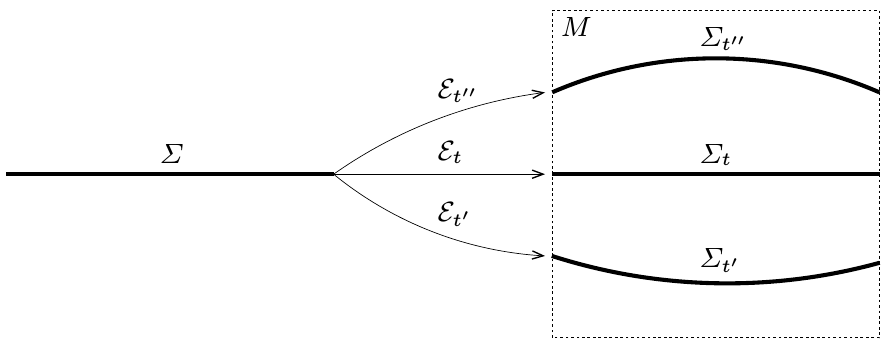
\includegraphics[width=0.7\textwidth]{FoilM.png}
\caption{Separación de la variedad $M$ mediante una familia, de un único parámetro, de encajes $\varepsilon_t$ de 3-variedades $\Sigma$ en $M$. $\Sigma_t$ es la imagen en $M$ de $\Sigma$ bajo $\varepsilon_t$.}
\label{fig:FoilM}
\end{figure}


Supongamos que tenemos una estructura de espacio-tiempo, es decir, una variedad diferenciable $M$ de dimensión cuatro y métrica $g_{\mu\nu}$ que se puede <<separar>> mediante una familia $\{\Sigma_t\,|\,t\in\mathbb{R}\}$ de hojas espaciales (hipersuperficies espaciales). Es decir, que para número $t$ existe un <<encaje>> (\emph{embedding}) de una variedad fija $\Sigma$ de dimensión tres en $M$

\begin{equation*}
 \varepsilon_t\,:\,\Sigma\rightarrow M\,,
\end{equation*}
cuya imagen $\varepsilon_t(\Sigma)\subset M$ es $\Sigma_t$, una subvariedad de la variedad $M$. En la figura (\ref{fig:FoilM}) se muestra este procedimiento. Cada hoja tridimensional $\Sigma_t$ se corresponde con un instante de tiempo $t$, donde $t$ es un <<tiempo>> topológico, una forma de etiquetar los instantes de forma continua pero que no tiene nada que ver con el tiempo de los relojes.

Gracias a este mecanismo hemos logrado recuperar la noción de tiempo: podemos ver el espacio-tiempo ($M,g$) como una familia de espacios parametrizada por un único parámetro $t$. De esta forma, el espacio-tiempo se interpreta como una <<trayectoria de espacios>>.


\subsection{\textit{Quantum Geometrodynamics.}}

\subsection{Gravedad cuántica de bucles (\textit{Loop Quantum Gravity}).}

%
%
%
%
\section{Teoría de cuerdas.}

%
%
%
%
\section{Teorías de campo efectistas.} % Víctor
% Con la bibliografía que tenemos del señor ese casi que la ponemos como una sección más...

%
%
%
%
\section{Otras aproximaciones.} % Tú o yo
% Lo que fuera aquí sería el complementario de lo anterior. Quizás podría escindirse según las opciones que hubiera...

%
%
%
%
\section{Conclusiones y perspectivas de futuro.} % ¿Los dos?

%
%
%
%
\section{Bibliografía}
\bibliographystyle{ieeetr}
\bibliography{Referencias}
\nocite{*}

\end{document}
